\documentclass[12pt,a4paper]{article}
\usepackage[a4paper,left=2cm,right=2cm,top=2cm,bottom=4cm]{geometry}
\usepackage[utf8]{inputenc}
\usepackage[T1]{fontenc}
\usepackage{amsmath}
\usepackage[ngerman]{babel}
\usepackage{amssymb}
\usepackage{float}
\usepackage{graphicx}
\usepackage{titling}
\usepackage{nicefrac}
\usepackage{xcolor}

\definecolor{xsens}{RGB}{0,115,188}
\usepackage{sectsty}
%\chapterfont{\color{xsens}}  % sets colour of chapters
%\sectionfont{\color{xsens}}  % sets colour of sections


%%%%%%%%%%%%%%%%%% HEADER AND FOOTER
\usepackage{fancyhdr}
\setlength\headheight{40pt}
\renewcommand{\headrulewidth}{0pt}
\pagestyle{fancy}
\lhead{\thetitle}
\rhead{
\includegraphics[height=4em]{Logos/X-SENSORS-Logo_Slogan_EN_Transparent.png}}
\rfoot{\thepage}
\cfoot{}

\usepackage{lipsum}

\author{Mirco Huber}
\newcommand{\subtitle}{Messungen an 3 Prototypen, Vergleich mit Gefran SB-46}
\title{X-706: Erstuntersuchungen}
\begin{document}
	\begin{titlepage}
		\begin{figure}[H]
			\centering
			
\includegraphics[width=.5\linewidth]{Logos/X-SENSORS-Logo_Slogan_EN_Transparent.png}
		\end{figure}
		\vspace*{3cm}
		\begin{center}
			\Huge {\thetitle} \\\vspace*{.5cm}
			\small {\subtitle}
		\end{center}
		\vspace{12cm}
		\hspace{.6\linewidth} 
		\begin{tabular}{l}	
			\small{\theauthor} \\[.5pt]  
			\small{X-Sensors AG} \\ 
			\small{Landenbergerstrasse 13} \\
			\small{CH-8253 Diessenhofen} \\ [.5cm] 	
			\today
		\end{tabular}
	\end{titlepage}
	\section{Warmlaufverhalten}
	Das Warmlaufverhalten war schon beim analogen Sensor deutlich bemerkbar. Der Sensor erfährt thermische Spannungen, wenn die Speisung eingeschaltet wird. Bis sich die Temperatur und die daraus resultierenden Spannungen homogenisieren / stabilisieren, weisen die DMS eine Signaländerung auf, welche aufgrund der massiven Verstärkung (Fullscale bei 30$\mu\varepsilon$) auf dem Ausgangssignal deutlich sichtbar sind.\\
	Untenstehend ist das Warmlaufverhalten des unverspannten Sensors über einen Zeitraum von 30min abgebildet. Weiter wurde eine PT-1-Kurve mit der Charakteristik
	\begin{equation}
		u(t) = A\cdot(1-e^{-b\cdot t + c})+d
	\end{equation}
	mittels Least squares in die Messdaten gefittet. Daraus lässt sich eine Zeitkonstante $\tau$ von 85s ermitteln, womit sich das Signal nach $3\cdot \tau \approx 4.5$min stabilisiert hat.
	\begin{figure}[H]
		\centering
		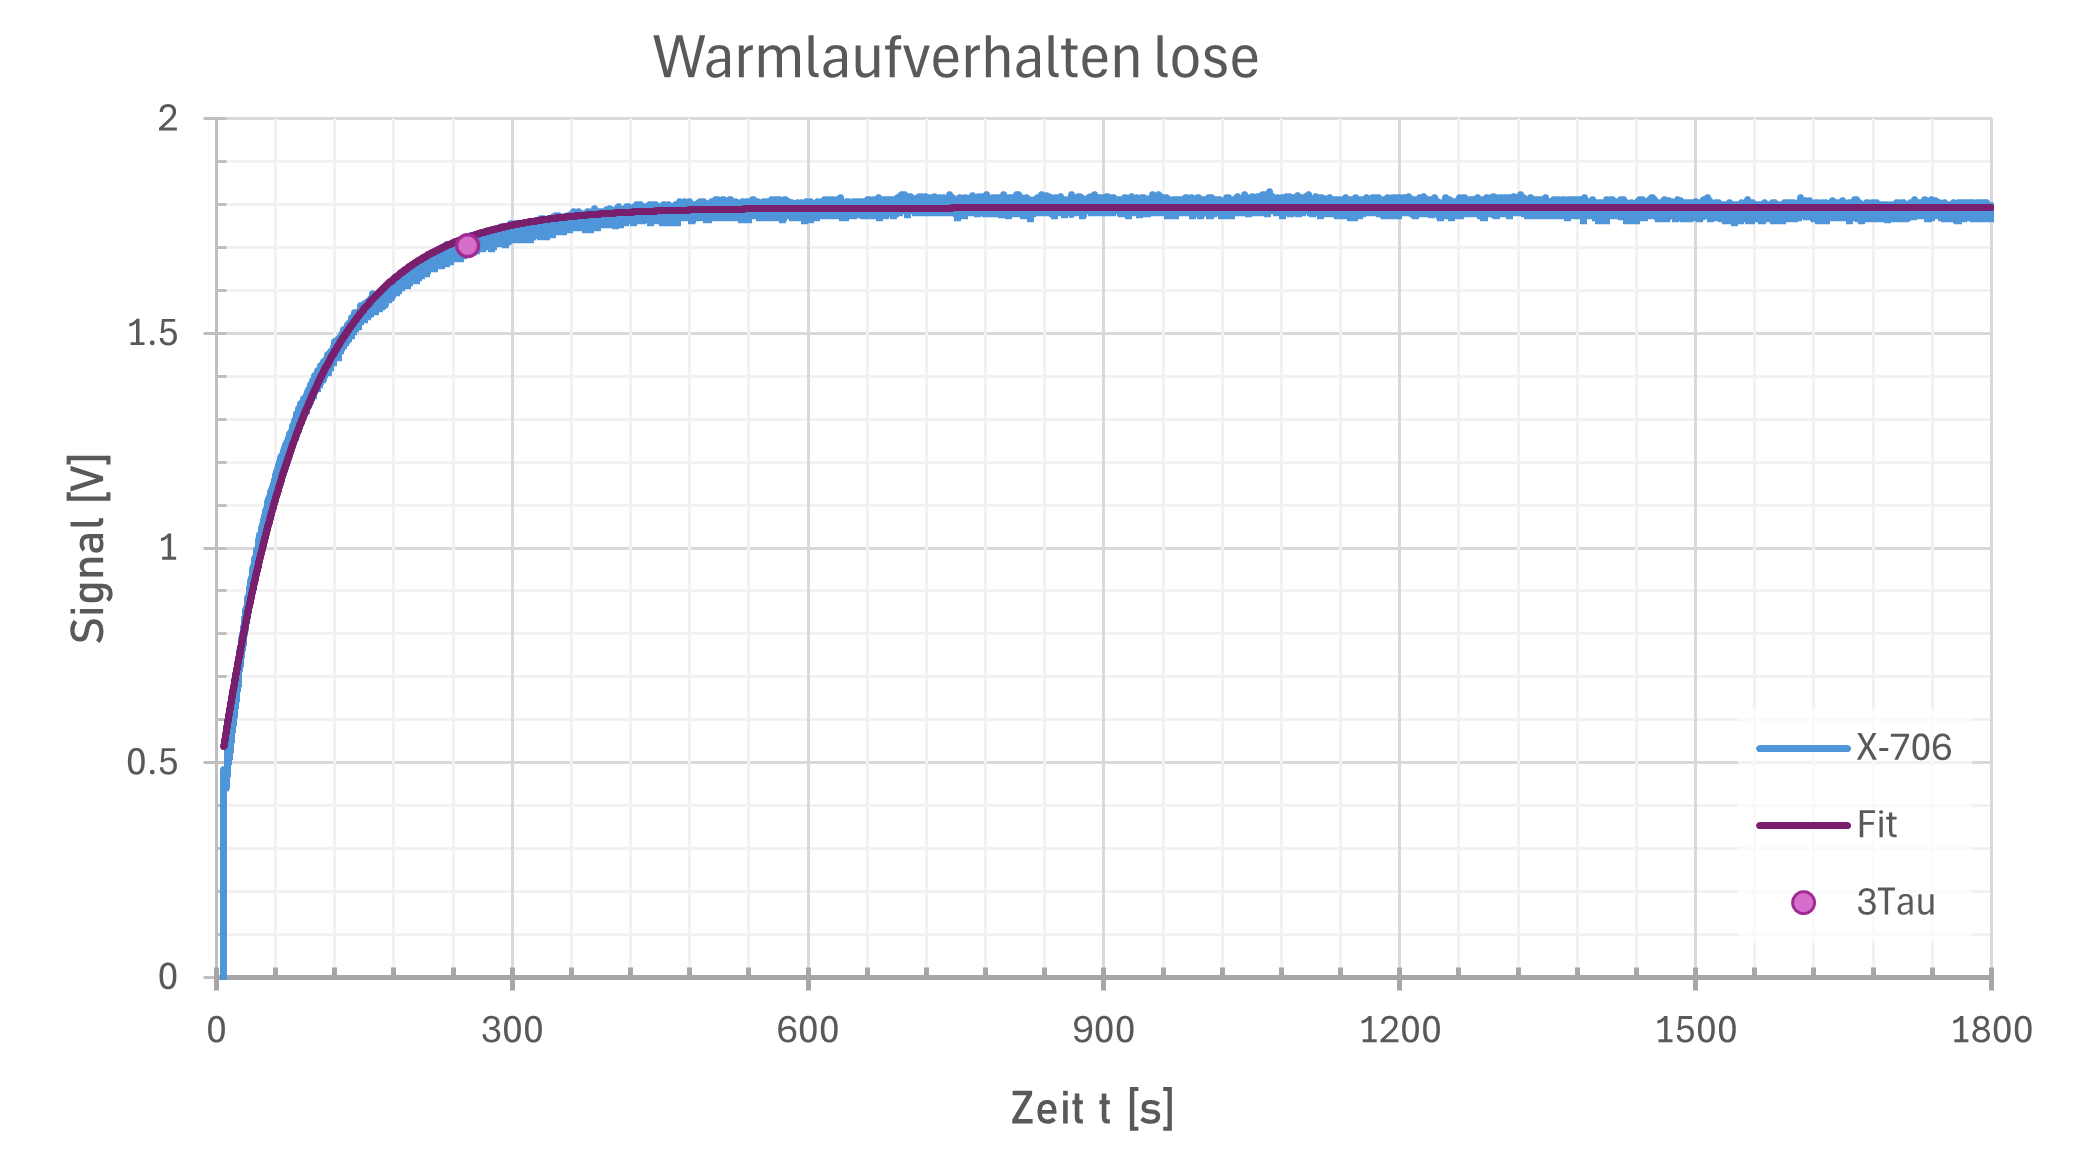
\includegraphics[width=1\linewidth]{Imgs/Warmlaufen_lose}
		\caption[Warmlaufverhalten lose]{Warmlaufverhalten lose}
		\label{fig:warmlaufenlose}
	\end{figure}\noindent
	Beim betrachten der zeitlichen Ableitung dieses Drifts fällt auf, dass die Signal-Änderung pro 10 Sekunden bereits 30 Sekunden nach dem Einschalten der Speisung unter 0.1$\nicefrac{V}{10s}$ beträgt. Wird also vor jedem Zyklus tariert und dauert ein Zyklus weniger als 10s, liegt der Nullpunkt-Drift 30 Sekunden nach anlegen der Speisespannung bei rund 1\% (0.1V bezogen auf 9.5V Fullscale).
	\begin{figure}[H]
		\centering
		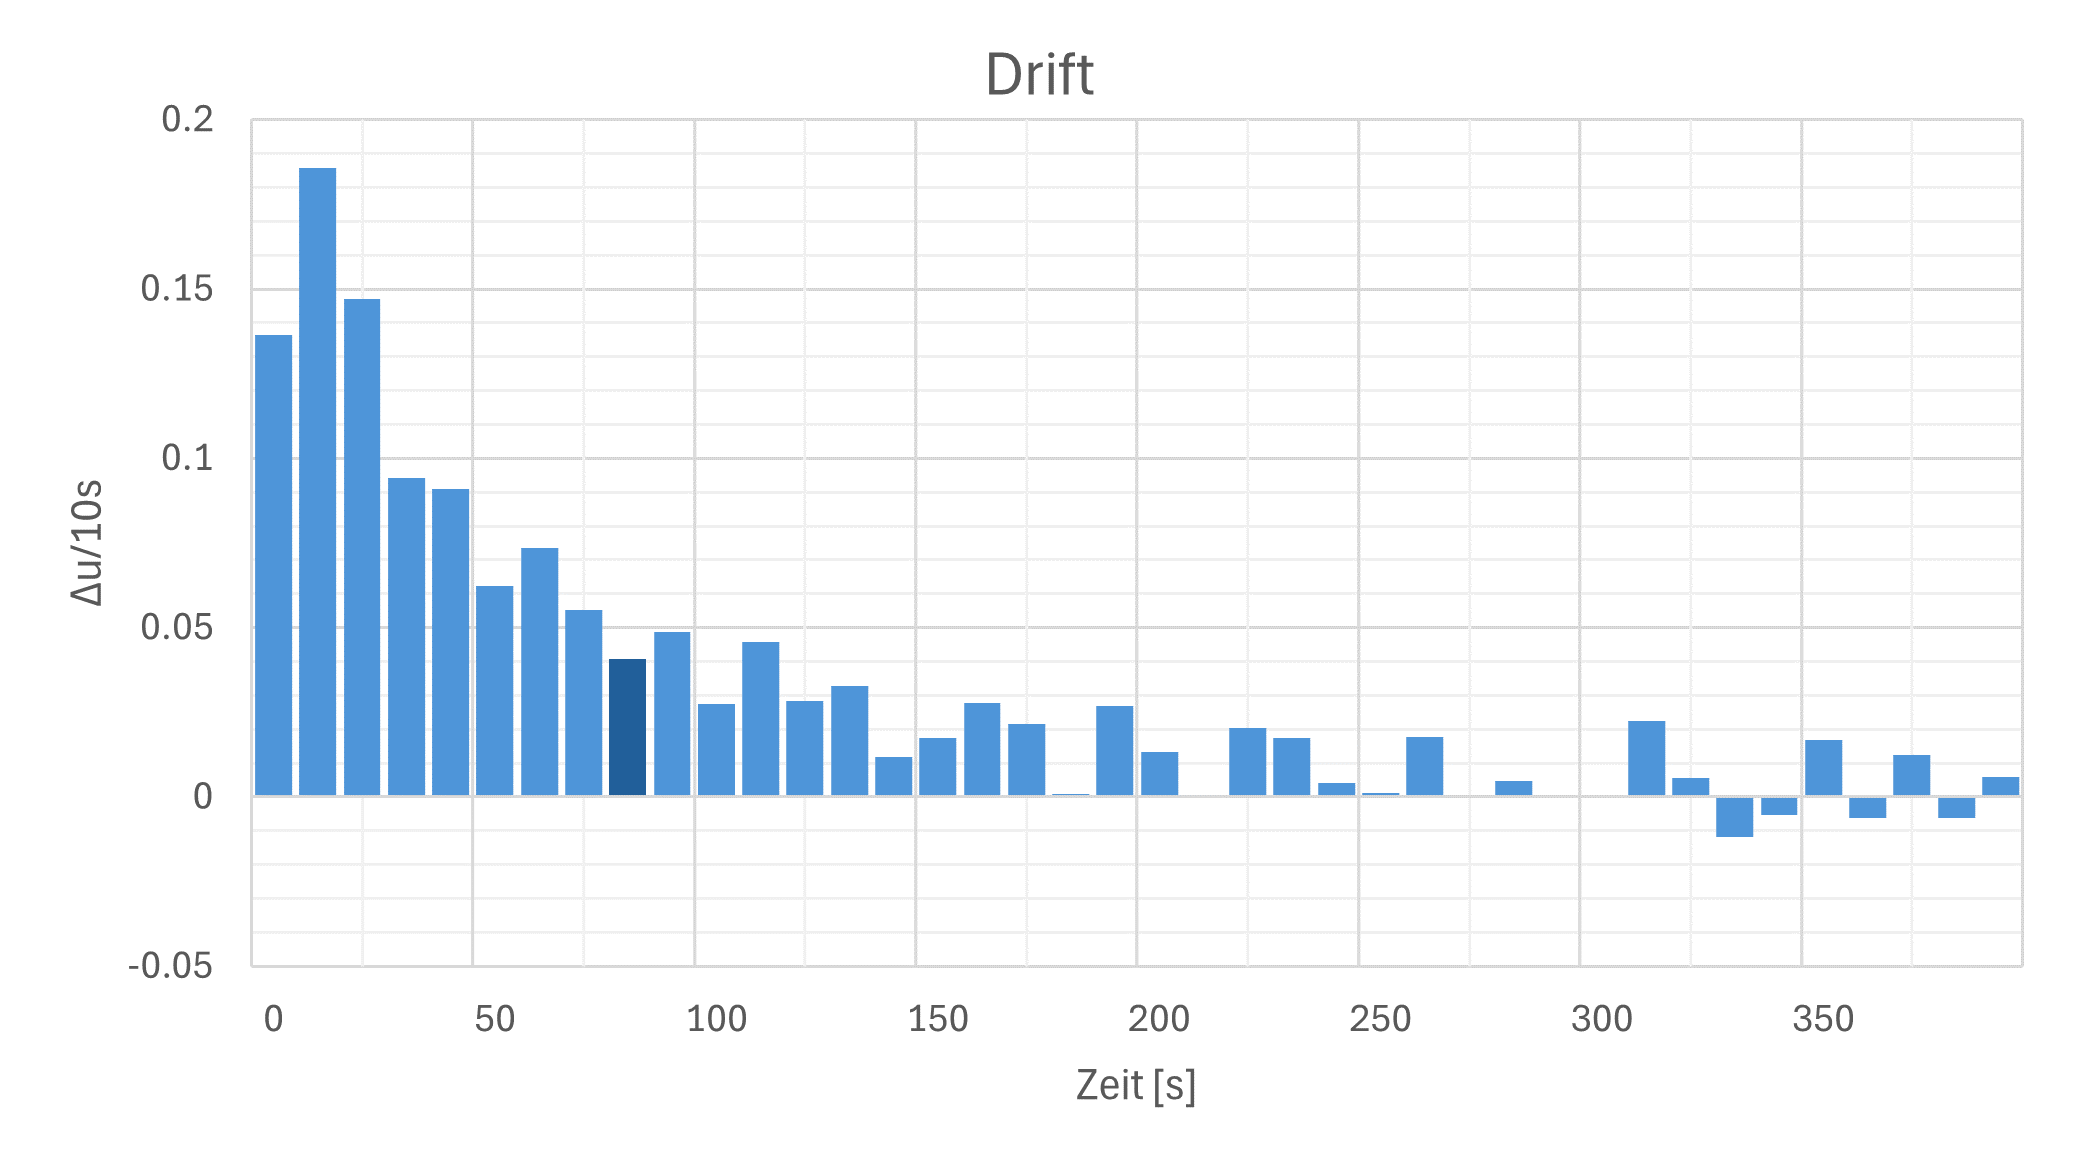
\includegraphics[width=1\linewidth]{Imgs/Warmlaufdrift_lose}
		\caption[Warmlauf-Drift pro 10 Sekunden ab Start]{Warmlauf-Drift pro 10 Sekunden ab Start: Ab 80s (dunkle Säule) ist der Drift vernachlässigbar ($\nicefrac{\Delta U}{\Delta t}\le 50mV$), wenn zyklisch / alle 10s tariert wird.}
		\label{fig:warmlaufdriftlose}
	\end{figure}\noindent
	Zusammengefasst kummuliert sich der Drift ohne zyklische Tarierung in den ersten rund 5 Minuten zu einem Offset von $\approx 1.3V$. Wird mindestens alle 10s tariert, beläuft sich der zeitliche Drift 30s nach Einschalten der Speisung auf maximal 0.1V, mit zunehmender Dauer kleiner werdend, bis er im Bereich des Rauschens liegt ($\pm 30 mV$)
	\section{Untersuchung aufgespannter Sensor}
	Bisherige Messungen wurden in unverschraubtem Zustand durchgeführt. Für alle kommenden Untersuchungen wurde unten dargestellter Testaufbau verwendet: X-706 und SB-46 wurden auf einer Zugstange mit den vorgeschriebenenen Drehmomenten (SB-46: 7Nm, \textbf{X-706: 5Nm}) aufgeschraubt. Sie wurden parallel von einem Labornetzteil gespiesen und die Tarier-Leitungen sind parallel geschaltet, womit die Sensoren simultan tariert werden können.
	\begin{figure}[H]
		\centering
		\includegraphics[width=0.5\linewidth]{"Imgs/Aufbau Zugstange"}
		\caption{Versuchsaufbau ``aufgespannt'' auf Zug-Prüfmaschine}
		\label{fig:aufbau-zugstange}
	\end{figure}
	\subsection{Warmlaufverhalten in aufgeschraubtem Zustand}
	Der Sensor zeigt im aufgespannten Zustand einen massiven Drift in den ersten 3 Minuten nach einschalten der Speisung. Der thermische Effekt ist auf die zu Beginn inhomogene Wärmeverteilung zurückzuführen, welche mechanische Spannungen aufbaut und aufgrund der starken Verstärkung bei dem geringen Fullscale von $30ue$ auf das Siganl durchschlägt.
	\begin{figure}[H]
		\centering
		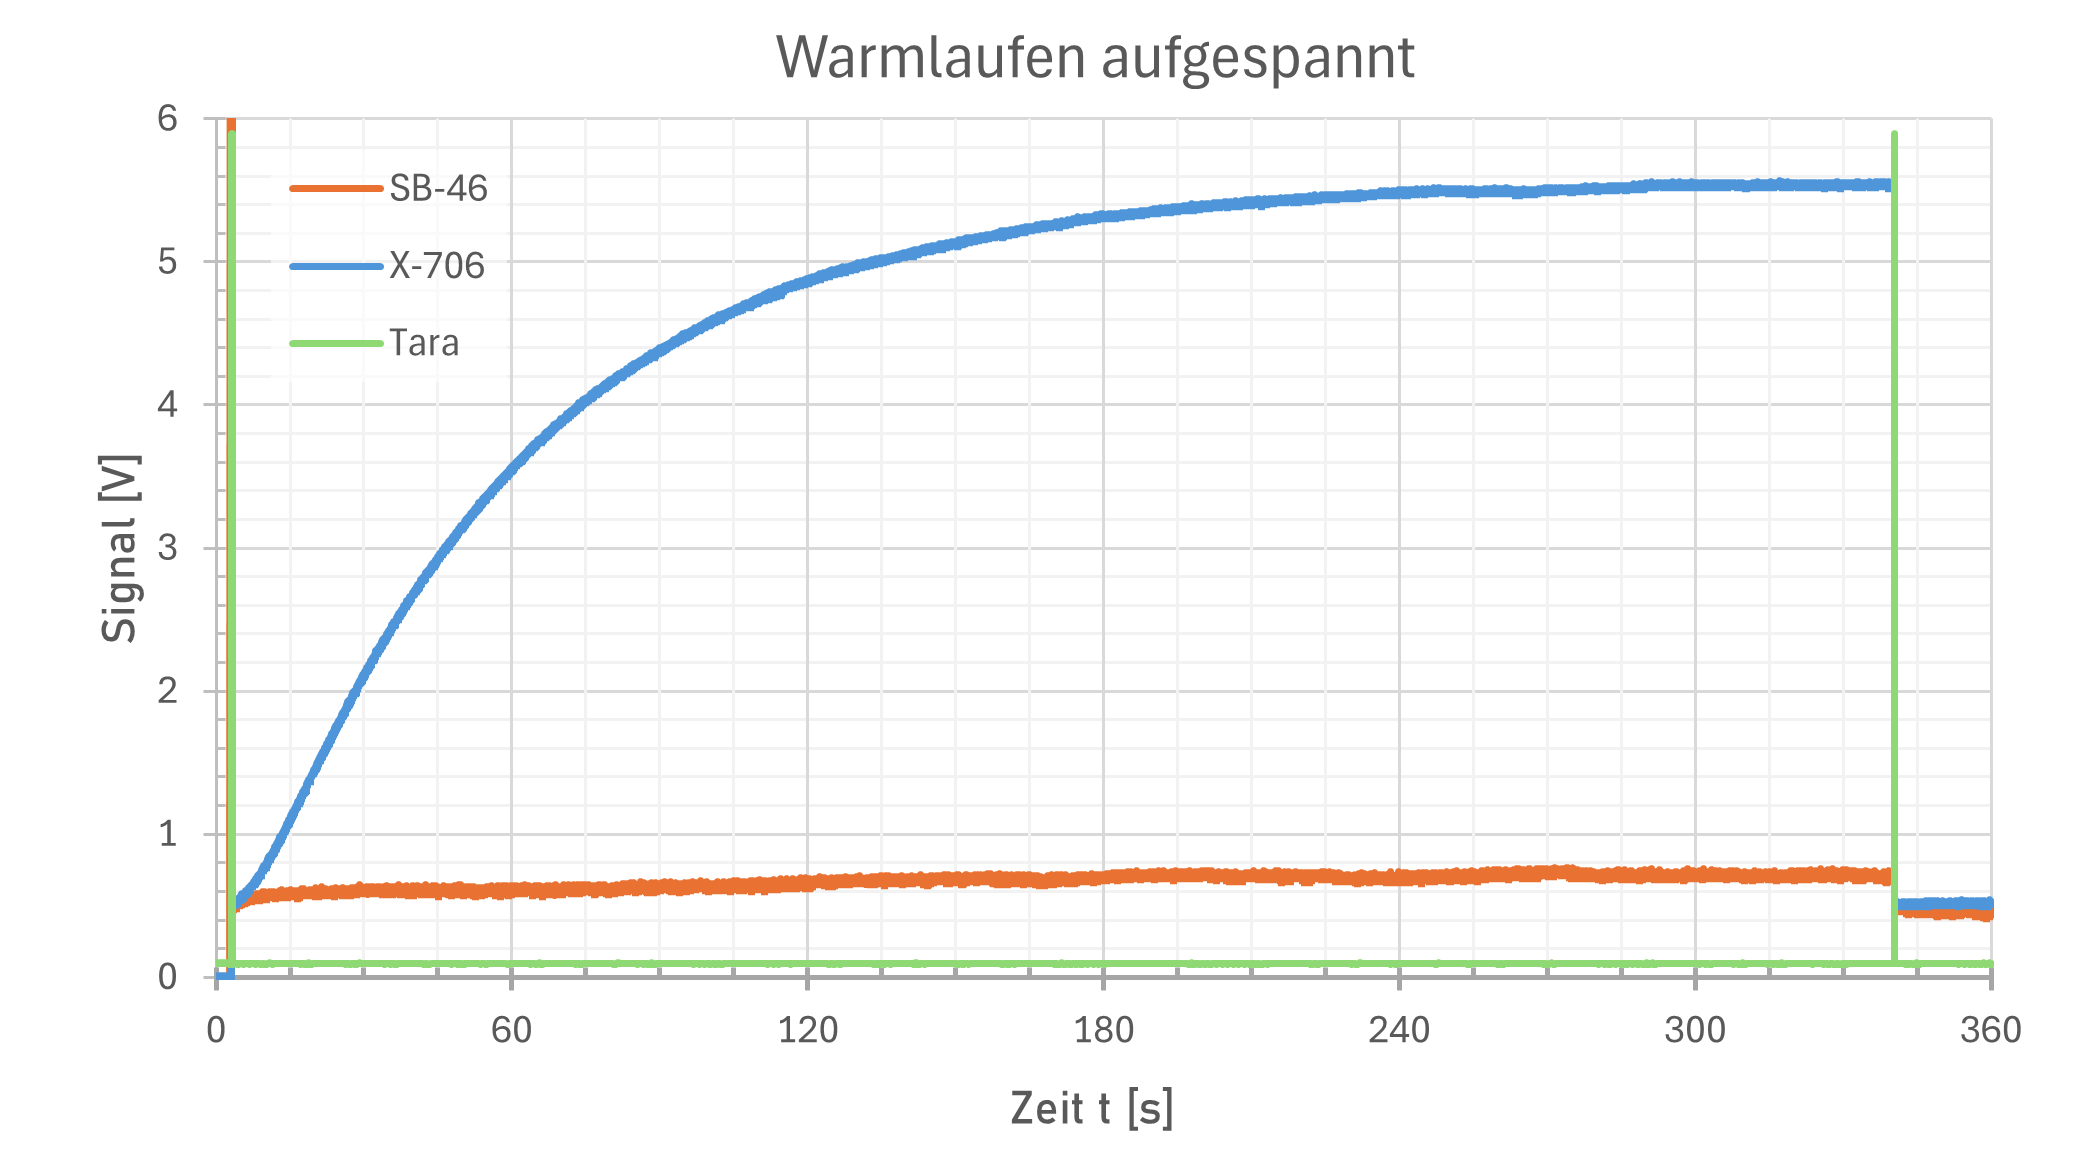
\includegraphics[width=1\linewidth]{Imgs/Warmlaufen_aufgespanntpng}
		\caption{Warmlaufverhalten in aufgeschraubtem Zustand}
		\label{fig:warmlaufenaufgespanntpng}
	\end{figure}\noindent
	Wird auch bei diesem Warmlaufverhalten die zeitliche Ableitung berücksichtig, zeigt sich, dass der Dirft für Zeitinkremente vom $\Delta t = 10s$ nach 2 Minuten auf unter 0.1V und nach 3 Minuten unter 50mV fällt. 
	\begin{figure}[H]
		\centering
		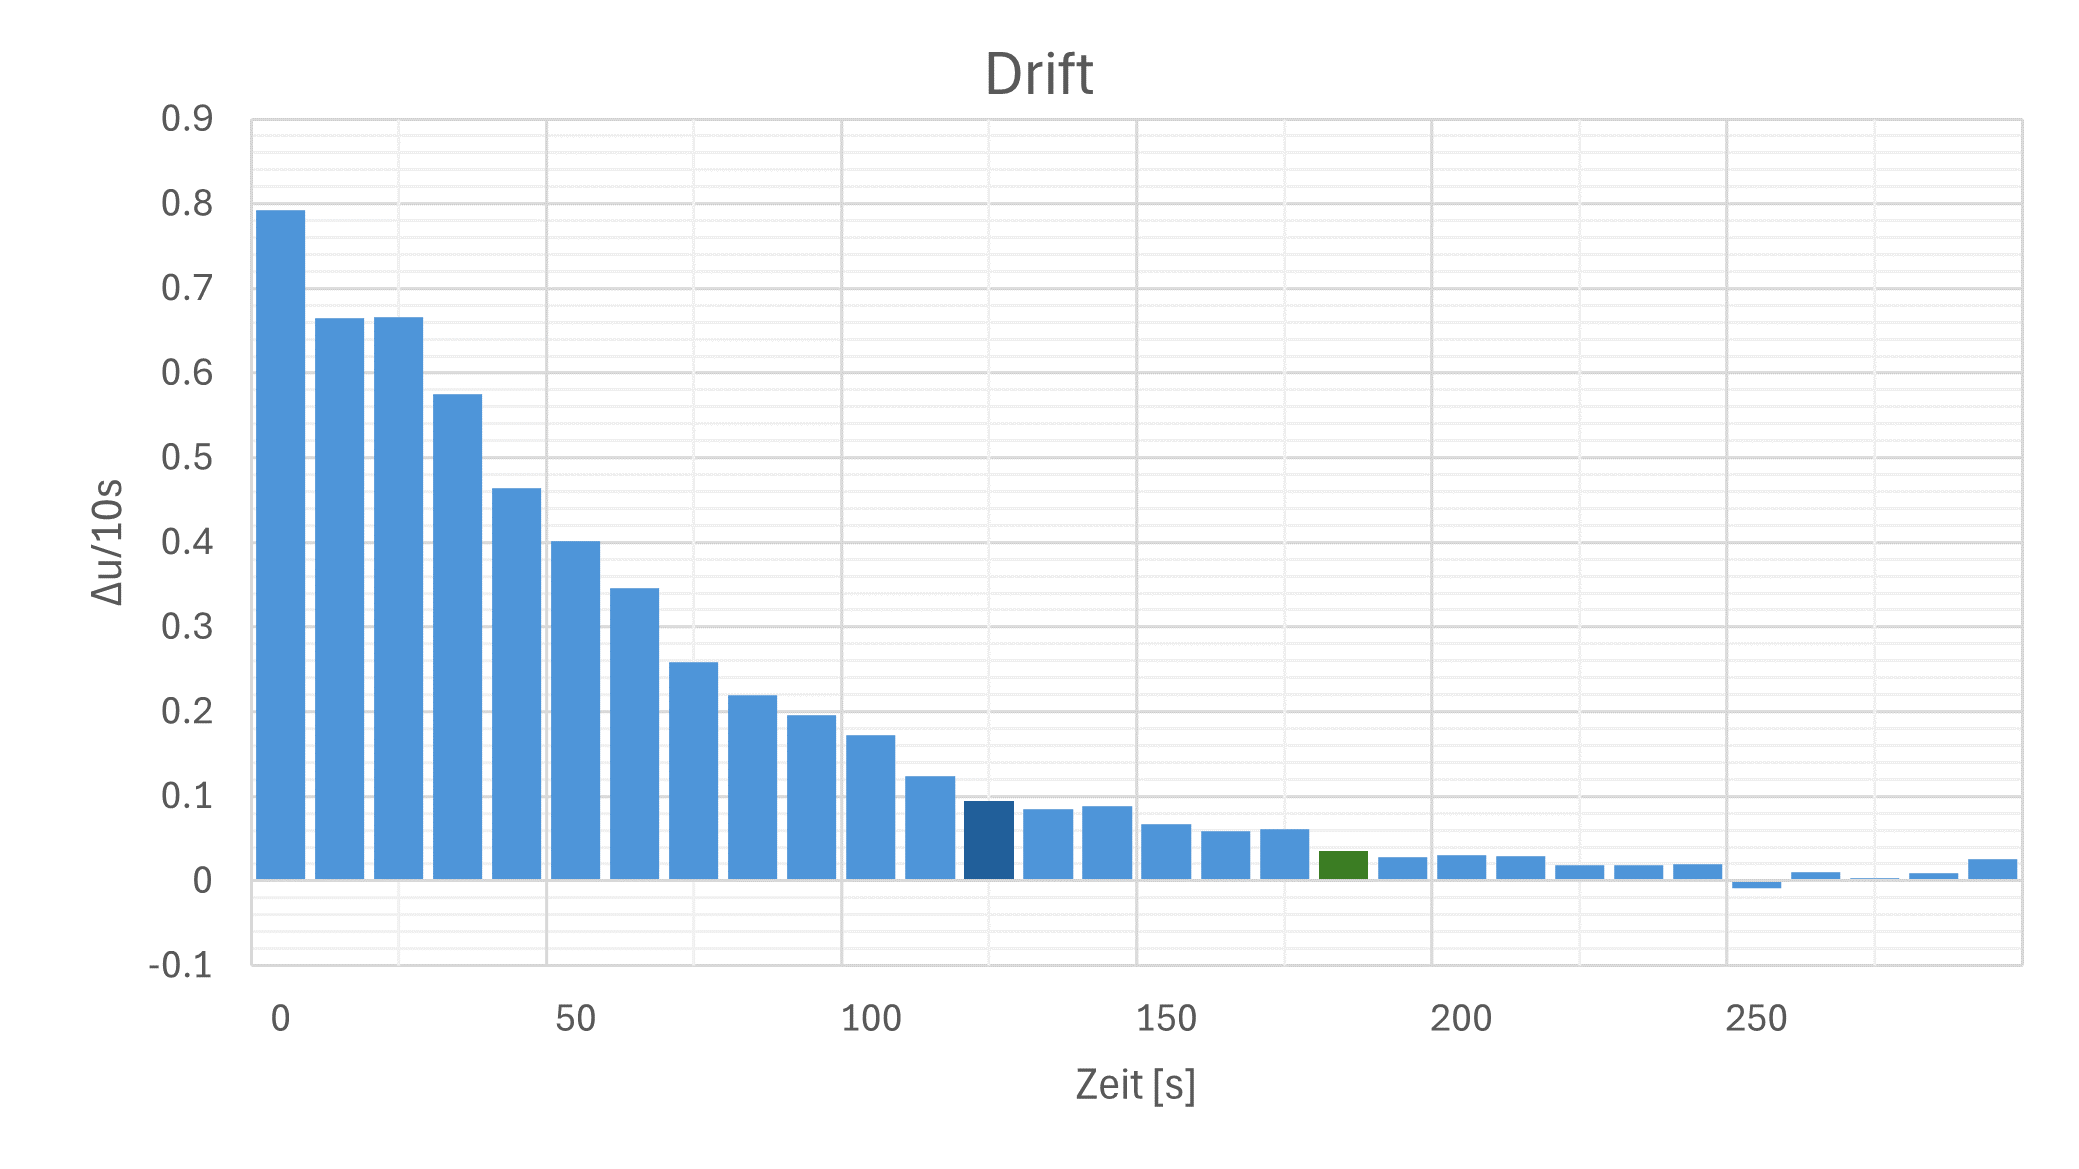
\includegraphics[width=1\linewidth]{Imgs/Warmlaufdrift_aufgespanntpng}
		\caption{Zeitliche Ableitung des Warmlaufdrifts: $\nicefrac{\Delta U}{\Delta t}$ nach 2min $<100\nicefrac{mV}{10s}$} (dunkelblaue Säule) und nach 3min $<50\nicefrac{mV}{10s}$
		\label{fig:warmlaufdriftaufgespanntpng}
	\end{figure}
	\subsection{Tarierdauer / -verhalten}
	Um das Tarierverhalten aufzuzeichnen, wurden die Sensoren auf der Zugstange vorbelastet (Signal $\ll 0V$) und anschliessend tariert. Die Signale wurden mit 10kHz abgetastet, das Tariersignal wurde auf das Intervall [0,1] skaliert.
	\begin{figure}[H]
		\centering
		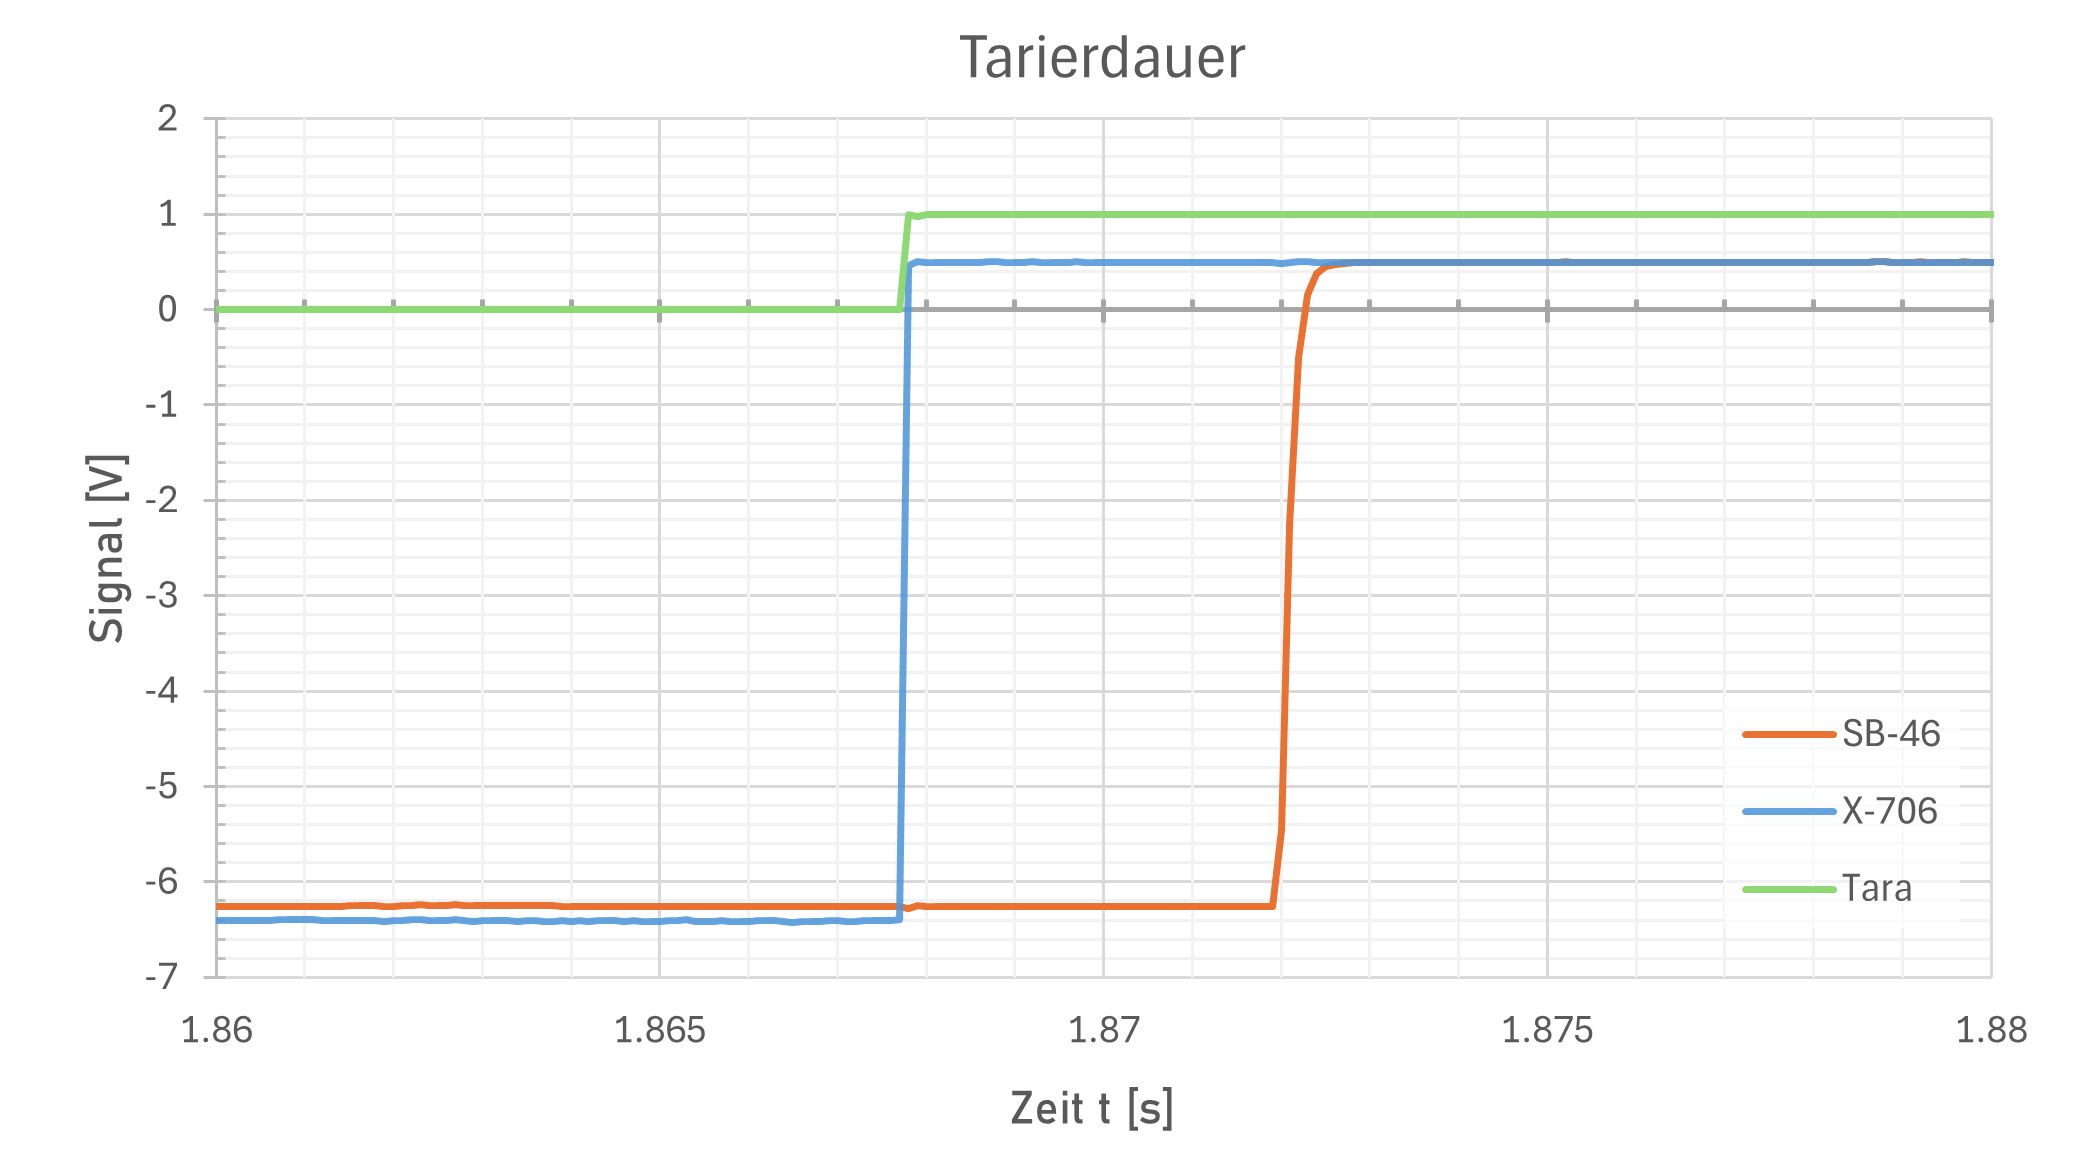
\includegraphics[width=1\linewidth]{Imgs/Tarierdauer}
		\caption{Direktvergleich Tarierdauer bei simultan angelegtem Tariersignal}
		\label{fig:tarierdauer}
	\end{figure}\noindent
	Die Abbildung \ref{fig:tarierdauer} zeigt, dass der neue Print im  $\mu s$-Bereich tariert und den Signalausgang bei steigender Flanke auf 0.5V setzt. Das Ausgangssignal ist fixiert, solange das Tariersignal \textit{HIGH} ist. Das Rauschverhalten während anliegendem (\textit{HIGH}) und nach gelöstem (\textit{LOW}) Tariersignal ist in Abbildung \ref{fig:rauschentaravorgang} visualisiert.
	\begin{figure}[H]
		\centering
		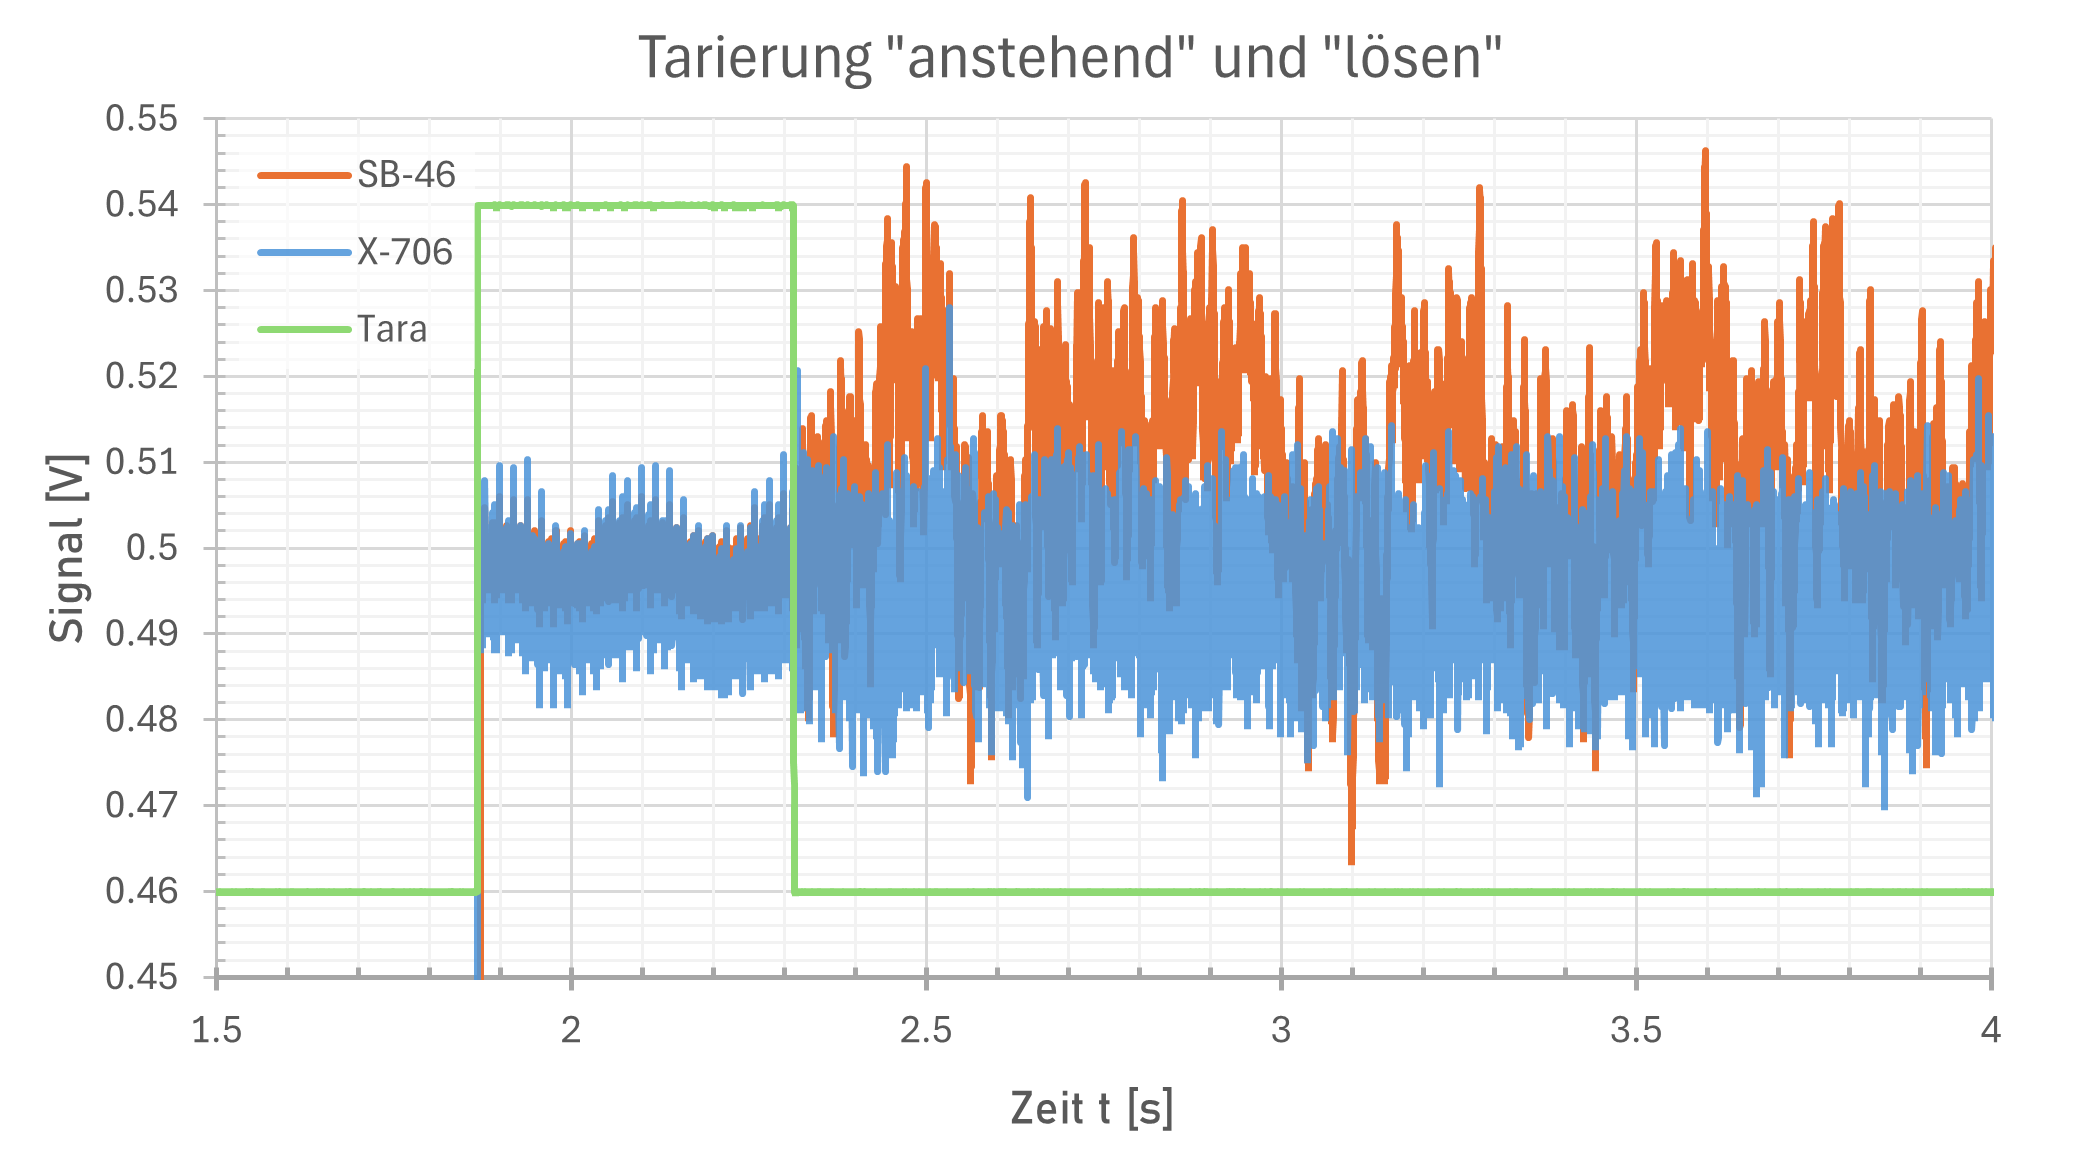
\includegraphics[width=1\linewidth]{Imgs/Rauschen_taravorgang}
		\caption{Rauschverhalten während Tariervorgang}
		\label{fig:rauschentaravorgang}
	\end{figure}\noindent
	Die Messung wurde für den Vorgang \textit{Tarierung lösen} über einen Zeitraum von 10s wiederholt (Abtastrate 1kHz), um das Rausch- und Dirftverhalten besser zu analysieren. 
	\begin{figure}[H]
		\centering
		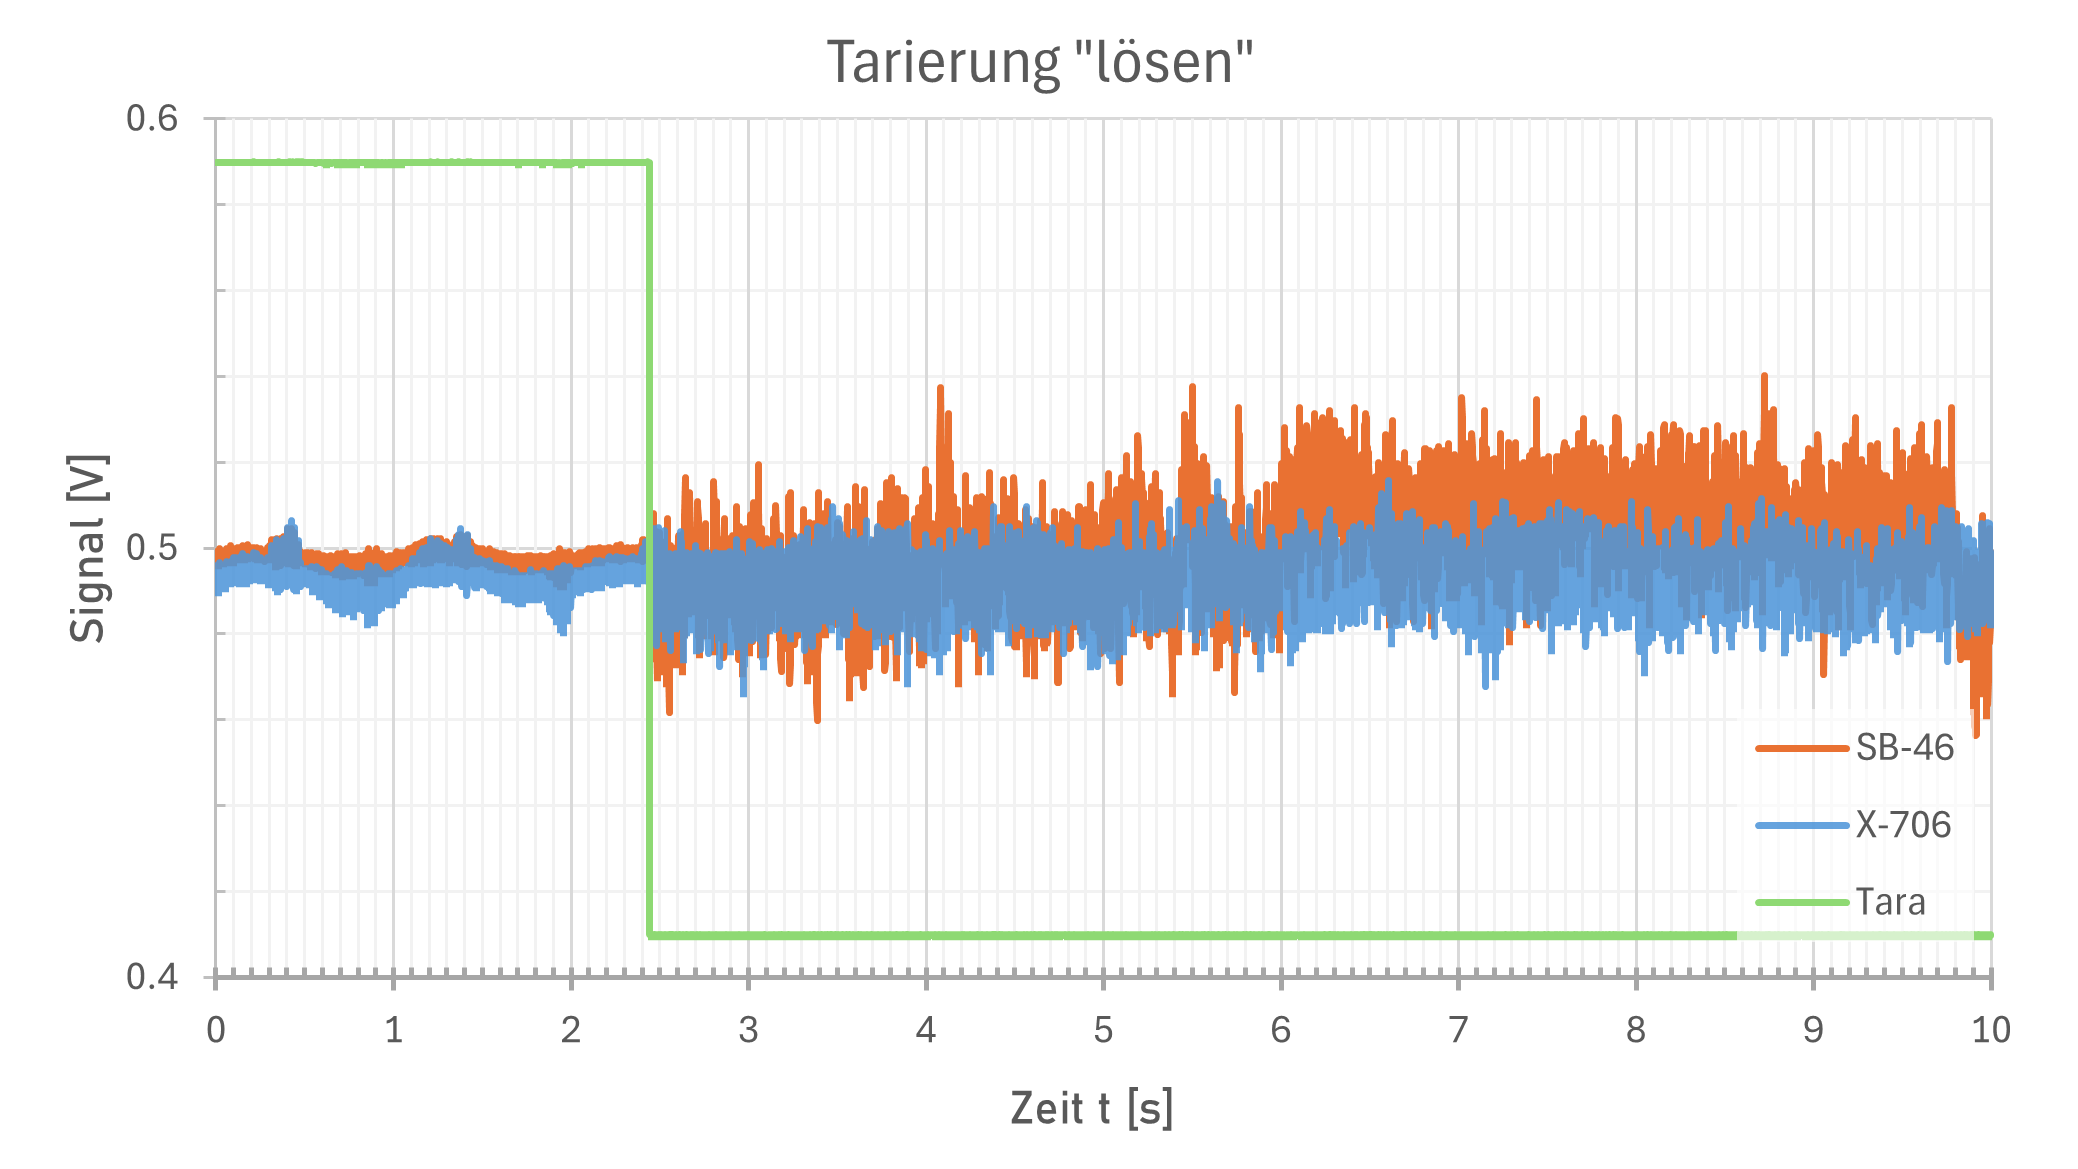
\includegraphics[width=1\linewidth]{Imgs/Tara_loesen}
		\caption{Zeitstabilität / Drift nach Tarierung}
		\label{fig:taraloesen}
	\end{figure}


\end{document}